\subsection{Shell Merger $\sim 1\mathrm{yr}$ to Core Collapse}\label{sec:CNOMerge}

Approximately one year before core collapse, the majority of models run at \gls{LowMetal} (using either mixing theory) showed a large shell merger, leading to an expansion. Notably though, the isotopes involved in the merger differed slightly between models (some occurring during O-burning, whilst others during or toward the end of C-burning).

Comparing Figures \ref{fig:KHD_Compare_Metal} (the lower diagram) and \ref{fig:KHD_Compare_Mix} also show how the merger style varies, with \ref{fig:KHD_Compare_Metal} expanding in two stages (at the end of Ne-burning and then when O-burning moves to a shell). 

Such a difference may, however, be numerical, since the models are equal in mixing theory, metallicity and resolution, meaning further investigation is needed to find the cause.

Figure \ref{fig:KHD_Compare_Mix} shows that, at the point of expansion, using \gls{MLT} leads to the creation of radiative pockets, whilst using \gls{TDC} leads to a more homogeneous convecting envelope. The timing of the expansion also differs, beginning earlier when using \gls{MLT} than with \gls{TDC}. 

The former effect could suggest that \gls{TDC} provides a more realistic representation of envelope convection than \gls{MLT}. 

The cause may be a smoothing effect created when treating \gls{TDC} in 1D, since fluid variables, 3D and local in nature, are approximated to 1D using averages (see Section \ref{sec:TDC}). 

The latter observation, meanwhile, is expected, since the short timescale and large uncertainty inevitably leads to timing inconsistencies between models during the late stages of evolution. 
%%%%

\begin{figure*}[t]
\begin{center}
    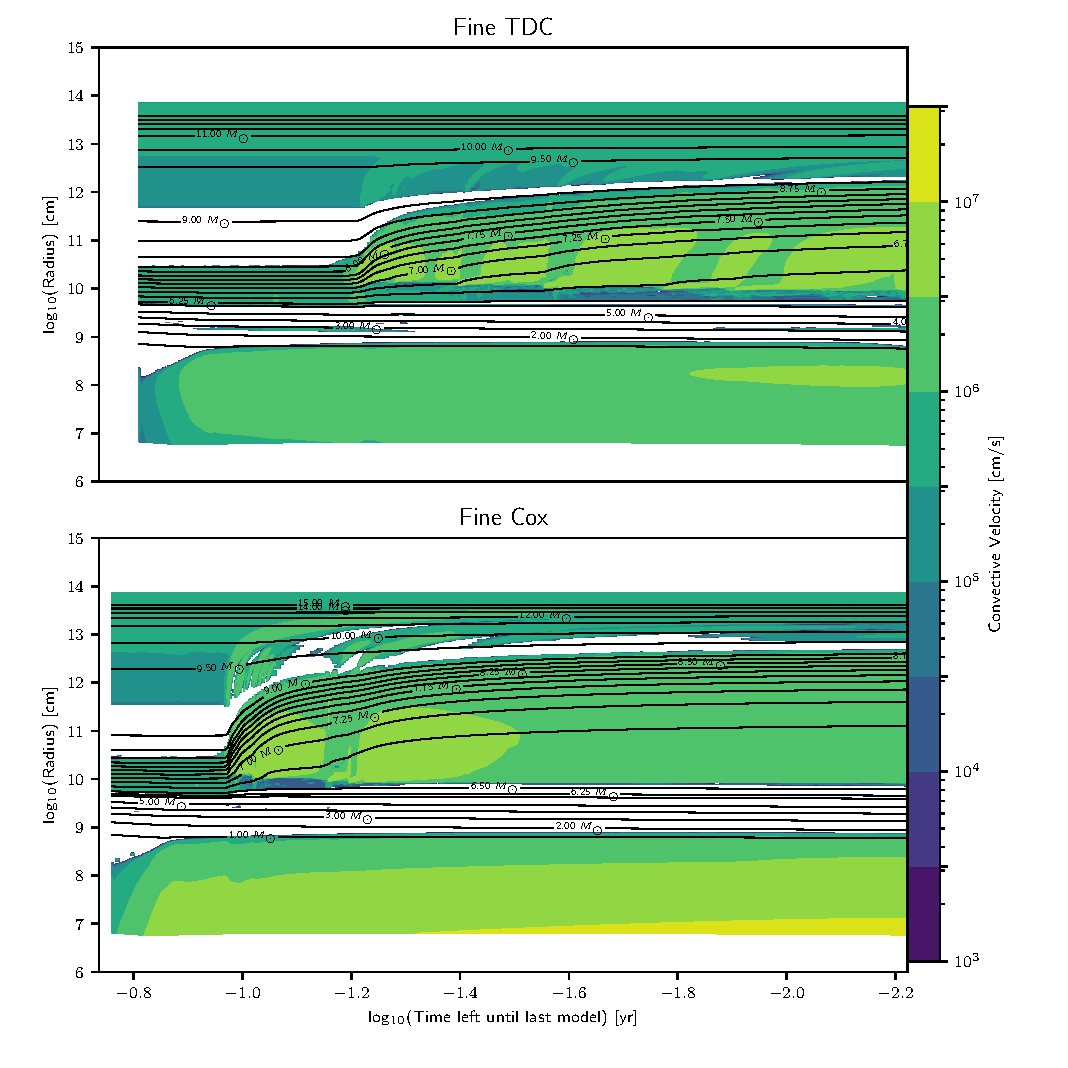
\includegraphics[width=0.9\linewidth]{Figures/KHD_Compare_Mix.pdf}
    \caption{Kippenhahn diagrams of radius (logarithmic) by time until core collapse, comparing an \gls{MLT} (lower) and \gls{TDC} (upper) run using short timestepping, focusing on a shell merger. Colour pertains to convective velocity.}
    \label{fig:KHD_Compare_Mix}
\end{center}
\end{figure*}

%%%%%%
% \begin{figure*}[t]
% \centering
% \begin{subfigure}{0.6\textwidth}
%     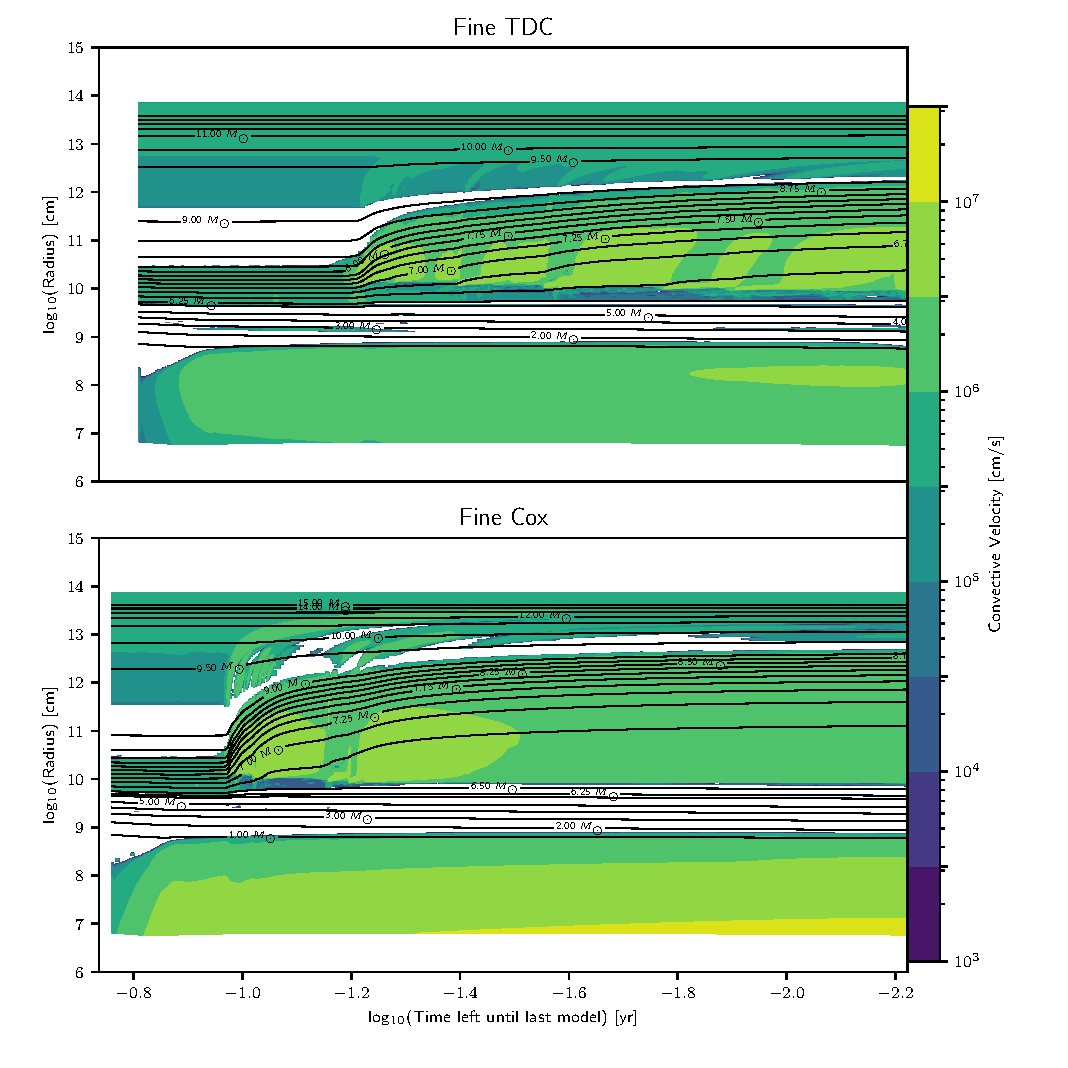
\includegraphics[width=\linewidth]{Figures/KHD_Compare_Mix.pdf}
%     \caption{Comparing an \gls{MLT} (lower) and \gls{TDC} (upper) run using short timestepping, focusing on a shell merger. Colour pertains to convective velocity.}
%     \label{fig:KHD_Compare_Mix}
% \end{subfigure}
% \hfill
% \begin{subfigure}{0.6\textwidth}
%     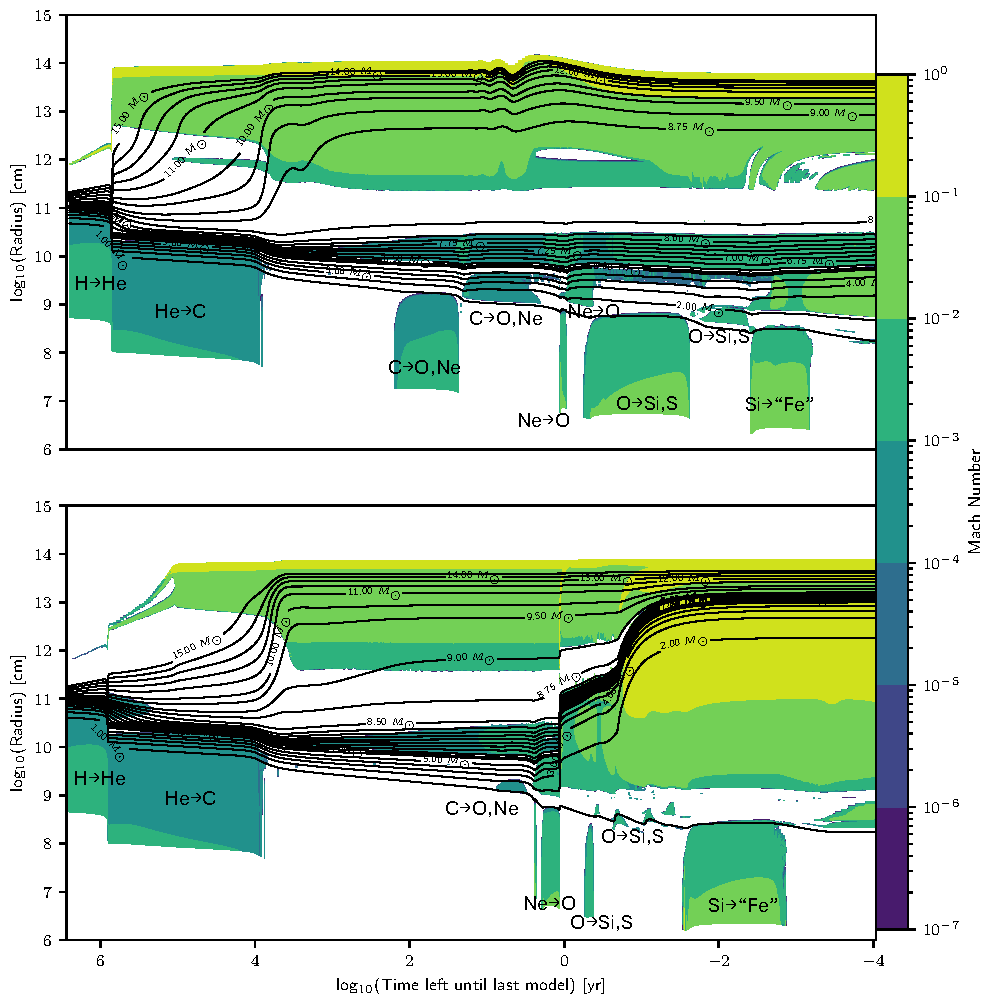
\includegraphics[width=\linewidth]{Figures/KHD_Compare_Metal.pdf}
%     \caption{Comparing a \gls{LowMetal} (lower) and \gls{SolarMetal} (upper) run using \gls{MLT} and short timestepping. Colour pertains to Mach number and label locations are based off of \citealp{Polls11}.}
%     \label{fig:KHD_Compare_Metal}
% \end{subfigure}
% \caption{Kippenhahn diagrams of radius (logarithmic) by time until core collapse.}
% \label{fig:KHDs}
% \end{figure*}